\documentclass[10pt, xcolor=table]{beamer}
\usepackage{inputenc}
\usepackage{graphicx}
\usepackage {mathtools}
\usetheme{CambridgeUS}
\usecolortheme{dolphin}
\usepackage{booktabs}
\usepackage{lscape}
\usepackage{caption}
\usepackage{tikz}
\usepackage{subcaption}
\usepackage{multicol}
\usepackage{xcolor}
\usepackage{pgfplots}
\usepackage{bm}
\usepackage{multicol}
\usepackage{adjustbox}
\usepackage{multicol}
\usepackage{cleveref}

\newcommand\dc[1]{\textcolor{blue}{#1}}
\setcounter{tocdepth}{3}
\pgfplotsset{compat=1.16}
\usepgfplotslibrary{external} 
\tikzexternalize

\newlength\figureheight
\newlength\figurewidth

\definecolor{myNewColorA}{RGB}{176,179,43}  % Yellow-Green
\definecolor{myNewColorB}{RGB}{42,111,74}   % Green
\definecolor{myNewColorC}{RGB}{52,142,209}  % Blue
\definecolor{myNewColorD}{RGB}{195,36,37}   % Red

\setbeamercolor*{palette primary}{bg=myNewColorC}
\setbeamercolor*{palette secondary}{bg=myNewColorB, fg=white}
\setbeamercolor*{palette tertiary}{bg=myNewColorA, fg=white}
\setbeamercolor*{titlelike}{fg=myNewColorA}
\setbeamercolor*{title}{bg=myNewColorA, fg=white}
\setbeamercolor*{item}{fg=myNewColorA}
\setbeamercolor*{caption name}{fg=myNewColorA}

\usefonttheme{professionalfonts}




\usepackage{natbib}
\usepackage{hyperref}
%------------------------------------------------------------
\titlegraphic{
    \begin{figure}
        \centering
        \begin{subfigure}[l]{0.45\textwidth}
            \centering
            
\includegraphics[width=2.5cm,height=1.5cm]{images/Logo_U.T.P.png}
        \end{subfigure}
        \hfill
        \begin{subfigure}[r]{0.45\textwidth}
            \centering
            
\includegraphics[width=2.5cm,height=2.5cm]{images/logo-maestria-scaled.jpg}
        \end{subfigure}
    \end{figure}
}

\setbeamerfont{title}{size=\Large\bfseries}
\setbeamerfont{subtitle}{size=\small}
\setbeamerfont{author}{size=\small}
\setbeamerfont{institute}{size=\footnotesize}

\title[Universidad Tecnológica de Pereira]{Stochastic Modeling of Multiple Streamflow Time Series in Colombian Based on Gaussian Processes}


 
\author[Julián David Pastrana-Cortés]{%
	\texorpdfstring{
		\begin{tabular}{c}
			\textbf{Author}: Julián David Pastrana-Cortés \\[1.5mm]
			\textbf{Director}: Álvaro Angel Orozco-Gutiérrez \\[1.5mm]
			\textbf{Co-director}: David Augusto Cardenas-Peña \\
		\end{tabular}
	}{Julián David Pastrana-Cortés}
}



\institute[Automatic]{Automatic Research Group}
\date{\today}

\AtBeginSection[]{
  \begin{frame}
    \vfill
    \centering
    \begin{beamercolorbox}[sep=8pt,center,shadow=true,rounded=true]{title}
      \usebeamerfont{title}\insertsectionhead\par%
    \end{beamercolorbox}
    \vfill
  \end{frame}
}

%------------------------------------------------------------

\begin{document}

\frame{\titlepage}
\section{Introduction}
\begin{frame}{Motivation}
	
	Understanding the implications of time series associated with hydrological variables, such as flow rates or reservoir levels, is essential for hydroelectric generation and the planning of other generation systems in Colombia
	
	\begin{figure}
		\centering
		\begin{subfigure}[b]{0.3\textwidth}
			\centering
			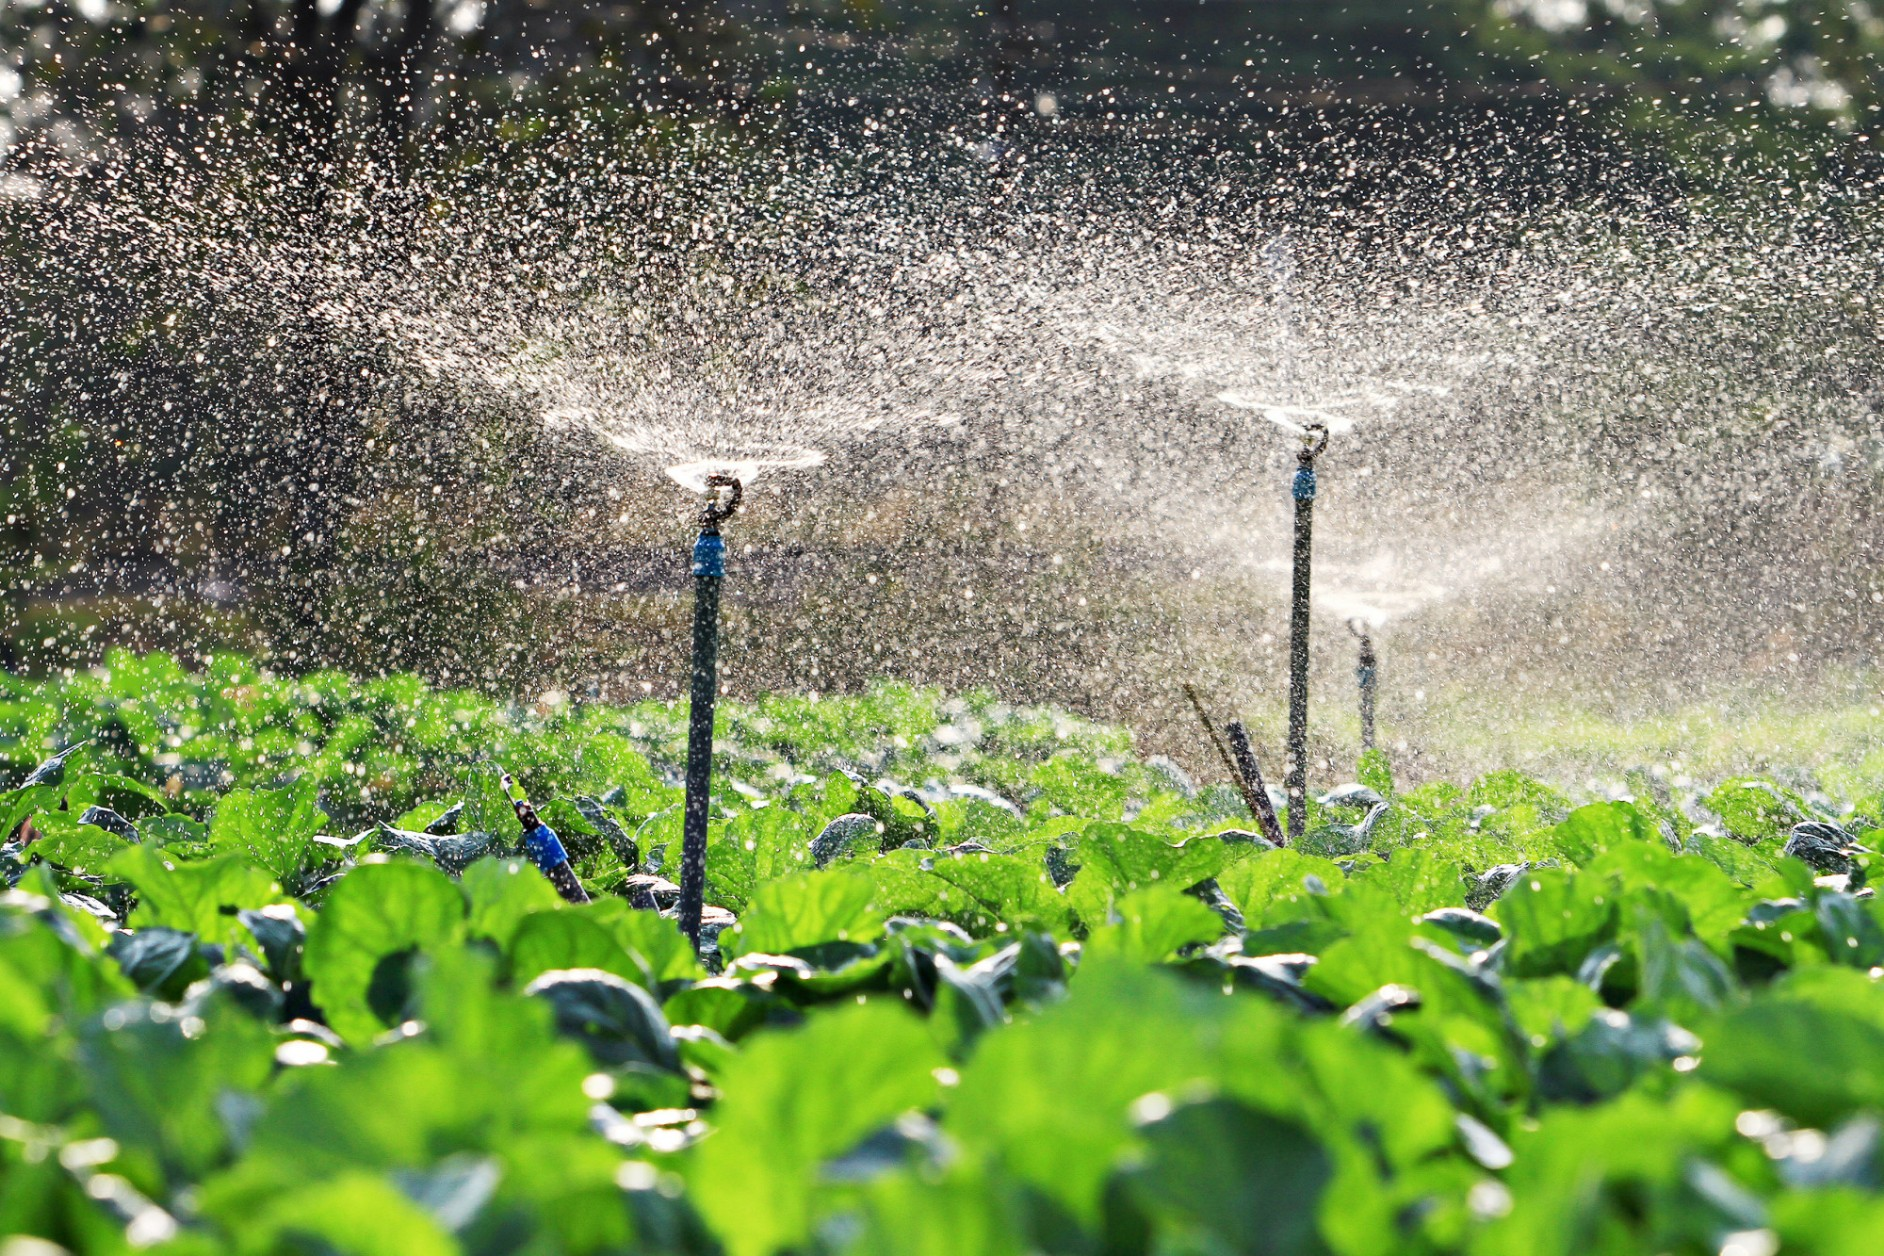
\includegraphics[width=\textwidth, height=4cm]{images/irrigation.jpg}
			\caption{Irrigation}
		\end{subfigure}
		\hfill
		\begin{subfigure}[b]{0.3\textwidth}
			\centering
			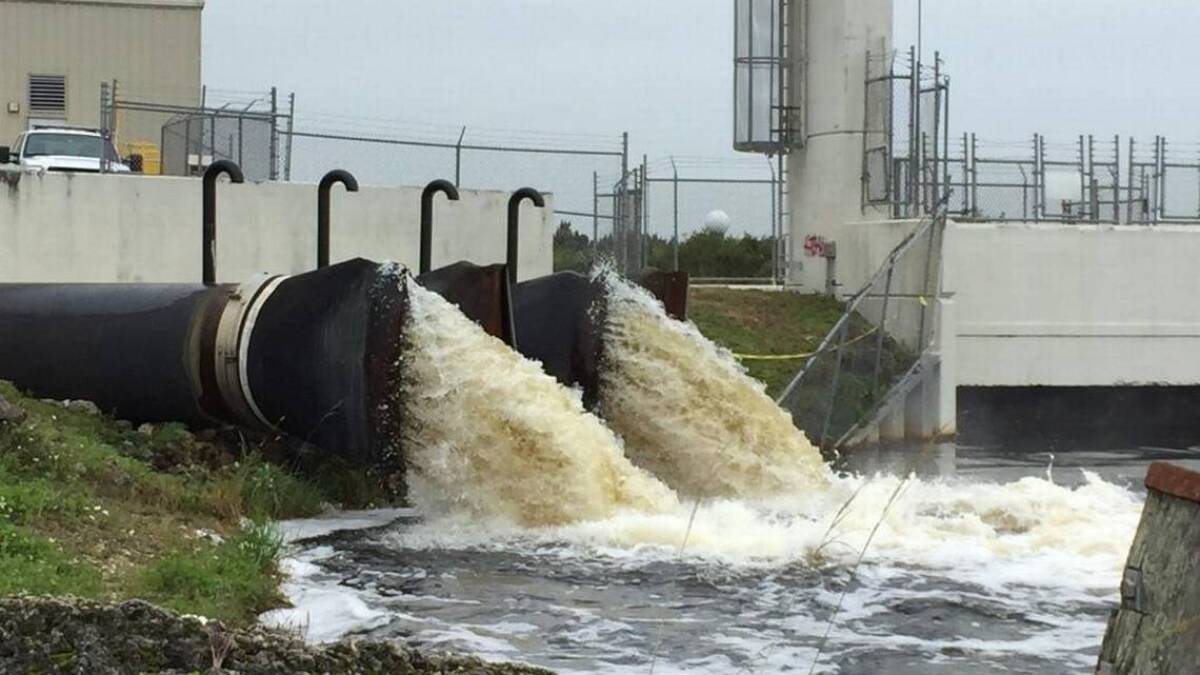
\includegraphics[width=\textwidth, height=4cm]{images/flood_control.jpeg}
			\caption{Flood control}
		\end{subfigure}
		\hfill
		\begin{subfigure}[b]{0.3\textwidth}
			\centering
			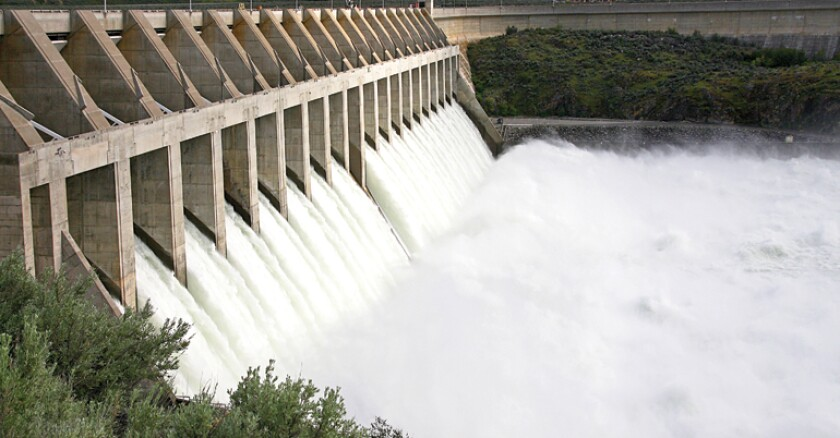
\includegraphics[width=\textwidth, height=4cm]{images/hydro_gen.jpeg}
			\caption{Hydropower generation}
		\end{subfigure}
		
	\end{figure}
\textcolor{myNewColorB}{\textbf{Challenges}}: non-linearities, high stochasticity, and complex water resource patterns.

\end{frame}

\begin{frame}
	\frametitle{The Importance of Hydrological Forecasting}
	
	Understanding hydrological processes has become increasingly critical in the field of natural resource management, anticipation capacity of extreme hydrological events such as droughts and heavy rainfall.
	
	\begin{figure}
		\centering
		\begin{subfigure}[b]{0.45\textwidth}
			\centering
			\includegraphics[width=\textwidth, height=4cm]{images/drought.jpg}
			\caption{Drought Condition}
		\end{subfigure}
		\hfill
		\begin{subfigure}[b]{0.45\textwidth}
			\centering
			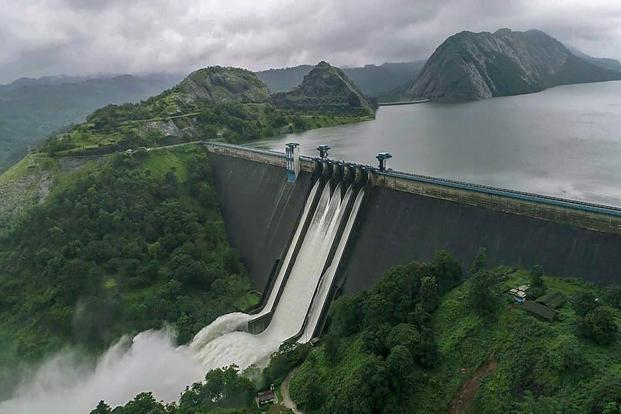
\includegraphics[width=\textwidth, height=4cm]{images/full_dam.jpg}
			\caption{Full Dam}
		\end{subfigure}
	\end{figure}
	
\end{frame}

\begin{frame}{The Proposed Model}
	A Gaussian Process (GP) is a Bayesian non-parametric model that provides not just point predictions but a full probability distribution, capturing uncertainty and enabling confidence intervals in time series forecasting.
	
	\begin{figure}
		\centering
		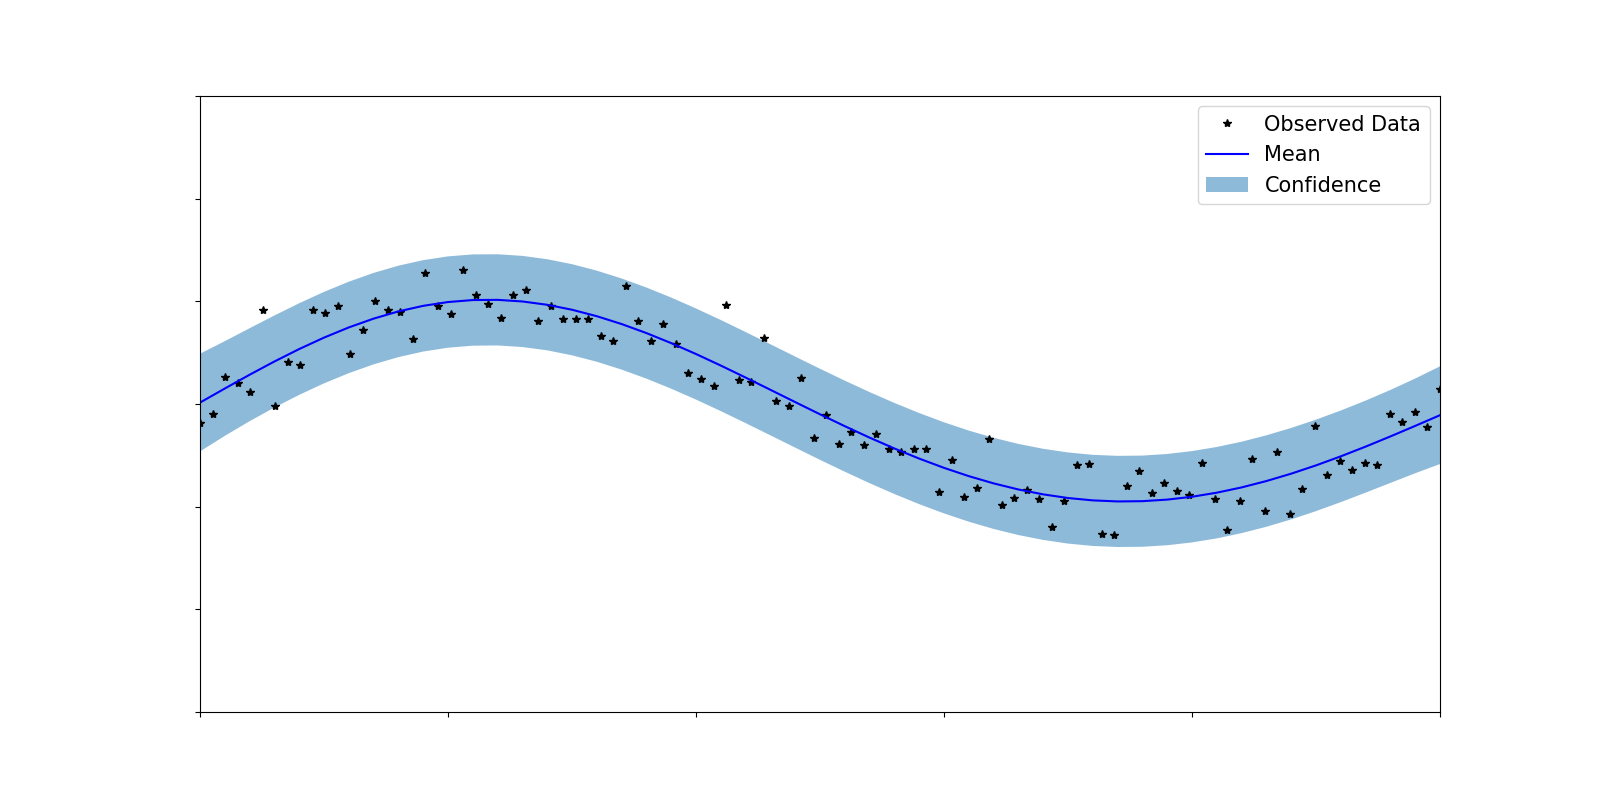
\includegraphics[width=\textwidth]{images/gpr.png}
	\end{figure}
\end{frame}

\section{Objectives}
\begin{frame}{General Objective}
	Develop a stochastic forecasting model for making multiple simultaneous predictions of hydrological time series, taking advantage of cross-correlations among the tasks to improve the performance keeping the scalability in its implementation for the short-term horizon.	
\end{frame}

\begin{frame}{Specific Objectives}
	\begin{itemize}
		\item Develop a model that allows the forecasting of hydrological time series, properly quantifying the uncertainty associated with each value within the prediction horizons.
		\item Design a multi-task forecasting methodology that captures and models cross-correlations between hydrological time series, to improve forecast accuracy within forecast horizons.
		\item Develop a multi-task prediction methodology that handles data constraints across reservoirs while maintaining high forecasting performance as measured by probabilistic metrics.
		
		% \item Develop a scalable multi-task prediction methodology across reservoirs, without compromising regression performance.
	\end{itemize}
\end{frame}

\section{The Dataset}
\begin{frame}{Problem Setting - Part 1}
	Consider a time-series vector of hydrological resources observed across all $D$ outputs at the $n$-th time instant, denoted as $\mathbf{v}_n \in \mathbb{R}^D$. Our model employs the entire sequence of resource vectors from time $n$ back to $n-T+1$ as input to predict the resource vector at the future time step $n+H$. Here, $T$ represents the model order, and $H$ denotes the prediction horizon. 
	
	Consequently, we define the input vector $\mathbf{x}_n$ as follows:
	
	\begin{equation*}
	\mathbf{x}_n = \begin{bmatrix} 
	\mathbf{v}_{n}^\top \\ 
	\mathbf{v}_{n-1}^\top \\ 
	\vdots \\ 
	\mathbf{v}_{n-T+1}^\top 
	\end{bmatrix} \in \mathbb{R}^{DT}
	\end{equation*}
\end{frame}

\begin{frame}{Problem Setting - Part 2}
	The target output vector $\mathbf{y}_n$ is defined as follows:
	
	\begin{equation*}
	\mathbf{y}_n = \mathbf{v}_{n+H}.
	\end{equation*}
	
	This formulation enables the model to leverage historical hydrological data for accurate future predictions. Accordingly, we build a dataset $\mathcal{D} = \{\bm{x}_n, \bm{y}_n\}_{n=1}^N = \{\mathbf{X}, \mathbf{y}\}$ comprising $N$ input--output pairs, where $\bm{x}_n \in \mathcal{X}\subset \mathbb{R}^{DT}$ represents the dimensional input space. The target function is a vector-valued function where $\bm{y}_n \in \mathbb{R}^{D}$ comprises the observations of all outputs (tasks) at the same input $\bm{x}_n$.
\end{frame}

\begin{frame}
	The hydrological forecasting task for validating the proposed model regressors considers time-series streamflow contributions data from 23 Colombian reservoirs.
	\begin{figure}[htbp]
		\centering 
		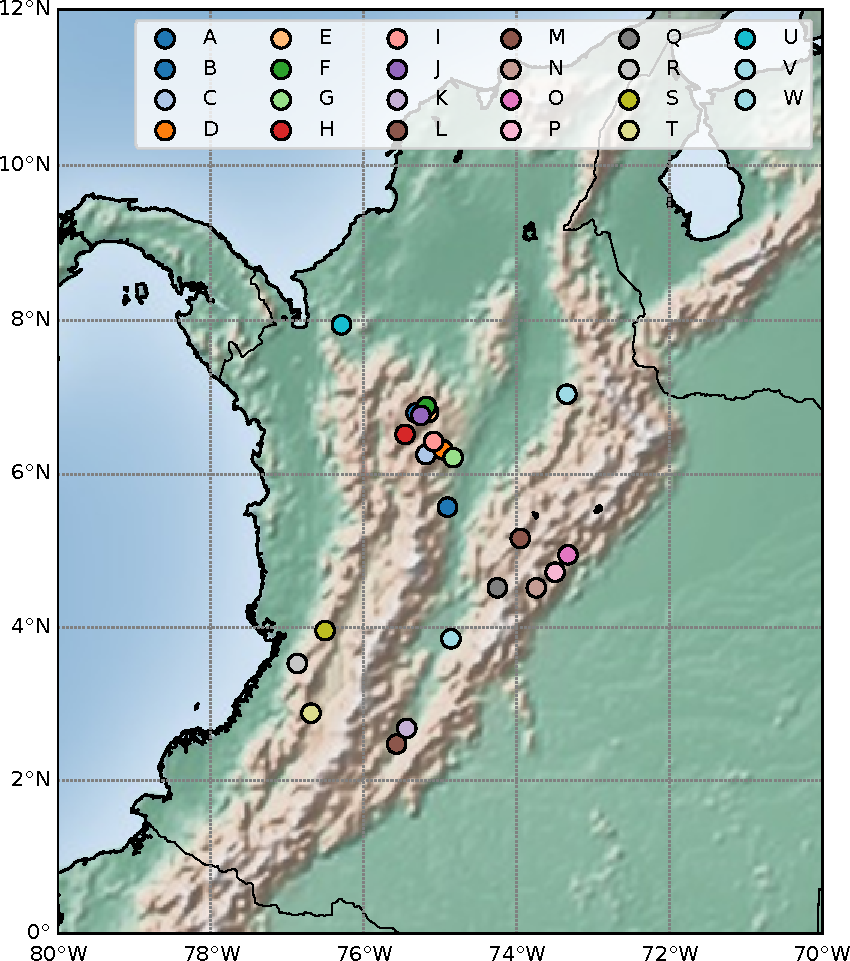
\includegraphics[height=0.5\textwidth]{images/colombiamap.pdf}
		\caption{Reservoir locations in Colombia.}
	\end{figure}
\end{frame}

\begin{frame}
	The dataset was selected due to the strong dependence of time series on weather patterns, which are closely tied to hydropower dispatch operations.
	
	\begin{figure}[htbp]
		\centering
		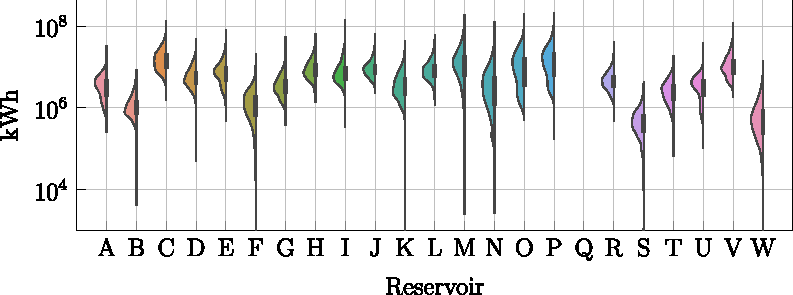
\includegraphics[height=0.25\textwidth]{images/ct_violinplot.pdf}
		\caption{Time-series Violin plot depicting the streamflow contribution for each reservoir within the dataset.}
	\end{figure}	
	
	These streamflow contributions were recorded daily from 1 January 2010 to 28 February 2022. While these contributions represent volumetric values, they are reported in kilowatt-hours (kWh) by the hydroelectric power plants.
\end{frame}



\section[Gaussian Process Regression]{Gaussian Process Regression: Bayesian Non-Parametric Model}
\begin{frame}
	In the context of the GP framework, the dataset $\mathcal{D}$ supports the learning of a random mapping function $\bm{f}(\cdot)$ that captures the relationship between $\bm{x}_n$ and $\bm{y}_n$. Thus, we pose a GP distribution over $\bm{f}(\cdot)$ as follows:
	\begin{equation}\label{mogp_notation}
	\bm{f}(\bm{x}) \sim  \mathcal{GP}\left(\bm{0},\, \bm{k}(\bm{x}, \bm{x}' \mid \bm{\theta})\right)
	\end{equation}
	where $\bm{f}: \mathcal{X} \rightarrow \mathbb{R}^D$ represents the vector-valued function responsible for mapping the input space, and {$\bm{k}: \mathcal{X} \times \mathcal{X} \rightarrow \mathbb{R}^{D \times D}$}
	symbolizes the cross-covariance matrix function, parameterized by vector $\bm{\theta}$. Adding i.i.d zero mean Gaussian noise to each task $\bm{\epsilon}$ with diagonal covariance matrix $\Sigma_\epsilon = \text{diag}\{\sigma^2_{Nd}\}_{d=1}^D \in \mathbb{R}^{D \times D}$ as a regularization term, the model prediction given by \Cref{mogp_notation} turns into $\bm{y}_n = \bm{f}(\bm{x}_n) + \bm{\epsilon}$, corresponding to a noise observation of the latent variable $\bm{f}$. 
\end{frame}

\end{document}



